\chapter{Testowanie rozwiązania}
\section{Środowisko testowe}
Wszystkie rozwiązania testowane będą przy użyciu następującego środowiska testowego:
\begin{description}
\item{Maszyna fizyczna:}
    \begin{itemize}
	\item CPU: \texttt{Intel(R) Core(TM)2 Quad CPU    Q9400  @ 2.66GHz} posiadający wsparcie dla wirtualizacji (\textit{VT-x})
	\item Pamięć RAM: \texttt{8G DDR2}
%%	\item OS: \texttt{Linux redraptor 3.18.1-gentoo \#7 SMP Wed Dec 31 02:04:37 CET 2014 x86\_64}
	\item OS: \texttt{Gentoo Linux 64bit, kernel 3.18.1}
	\item Platforma wirtualizacyjna: \texttt{KVM} (host)
    \end{itemize}
\item{Maszyna wirtualna na potrzeby kontenerów:}
    \begin{itemize}
	\item CPU: Mapowany z maszyny fizycznej. Przydział 3 rdzeni
	\item Pamięć RAM: \texttt{2G}
%%	\item OS: \texttt{Linux lxc 3.13.0-24-generic \#46-Ubuntu SMP Thu Apr 10 19:11:08 UTC 2014 x86\_64 x86\_64 x86\_64}
	\item OS: \texttt{Ubuntu Linux 64 bit, kernel 3.13.0-24-generic}
	\item Platforma wirtualizacyjna: \texttt{KVM} (guest), \texttt{LXC} (host)
    \end{itemize}
\item{Kontenery \texttt{LXC} do celów testowania aplikacji:}
    \begin{itemize}
	\item OS: Ubuntu linux. Jądra współdzielone z maszyną hostującą.
	\item Ustawienia \texttt{cgroups}: \texttt{lxc.cgroup.cpu.cfs\_quota\_us = 30000}
    \end{itemize}
\item{Maszyna wirtualna na potrzeby \texttt{LVS}:}
    \begin{itemize}
	\item CPU: Mapowany z maszyny fizycznej. Przydział 1 rdzeń
%%    	\item OS: \texttt{Linux mgr10 3.13.0-24-generic \#46-Ubuntu SMP Thu Apr 10 19:11:08 UTC 2014 x86\_64 x86\_64 x86\_64}
	\item OS: \texttt{Ubuntu Linux 64 bit, kernel 3.13.0-24-generic}
	\item Pamięć RAM: \texttt{192M}
    \end{itemize}
\end{description}
Aplikacje działające w \texttt{userspace}, tj. \texttt{apache, nginx, haproxy, php-fpm}, zostają uruchamiane w dedykowanych kontenerach \texttt{LXC}.
Usługi działające w warstwie jądra, tj. \texttt{LVS} zostają uruchomione na dedykowanej maszynie wirtualnej przy użyciu \texttt{KVM}.
\section{Wybór serwera WWW}
W rozdziale tym zostanie przedstawione zestawienie kilku testów wydajnościowych dwóch serwerów WWW.
\begin{itemize}
\item Apache2
\item Nginx
\end{itemize}
Przetestowane zostanie serwrowanie plików statycznych oraz treści dynamicznych PHP{.}\\
Wszystkie testy zostały przeprowadzone z wykorzystaniem 10 000 połączeń.\\
Wszystkie czasy zostały podane w milisekundach.
\subsection{Pliki statyczne}
Testy plików statycznych przeprowadzone zostaną przy użyciu dwóch plików HTML{.}
Jeden o rozmiarze 10 bajtów, drugi o rozmiarze 100 kilobajtów.

\begin{figure}
	\centering
	\begin{subfigure}[h]{0.3\textwidth}
		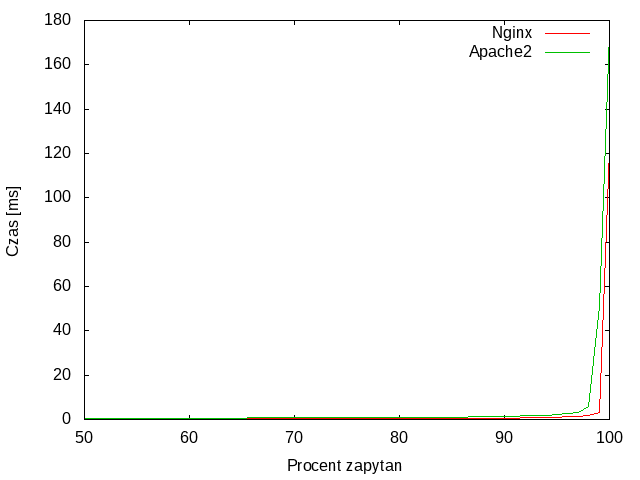
\includegraphics[width=\textwidth]{testy/wybor_index_maly_1.png}
		\caption{1 równoległe zapytanie}
	\end{subfigure}
	\begin{subfigure}[h]{0.3\textwidth}
		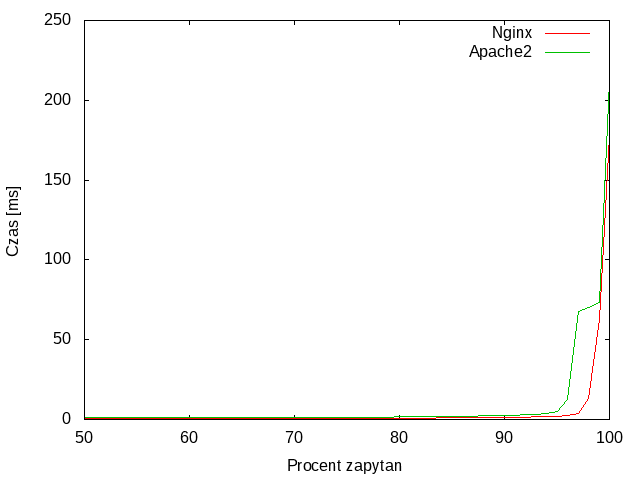
\includegraphics[width=\textwidth]{testy/wybor_index_maly_2.png}
		\caption{2 równoległe zapytania}
	\end{subfigure}
	\begin{subfigure}[h]{0.3\textwidth}
		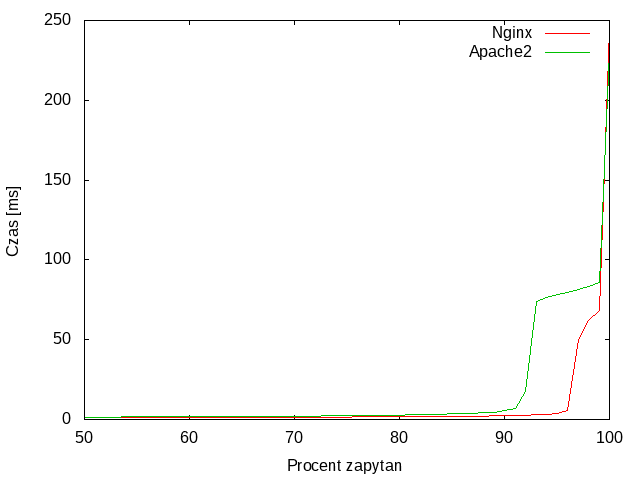
\includegraphics[width=\textwidth]{testy/wybor_index_maly_4.png}
		\caption{4 równoległe zapytania}
	\end{subfigure}

	\begin{subfigure}[h]{0.3\textwidth}
		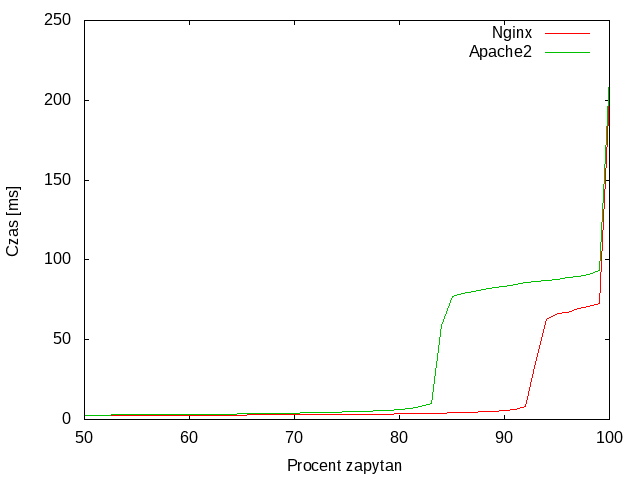
\includegraphics[width=\textwidth]{testy/wybor_index_maly_8.png}
		\caption{8 równoległych zapytań}
	\end{subfigure}
	\begin{subfigure}[h]{0.3\textwidth}
		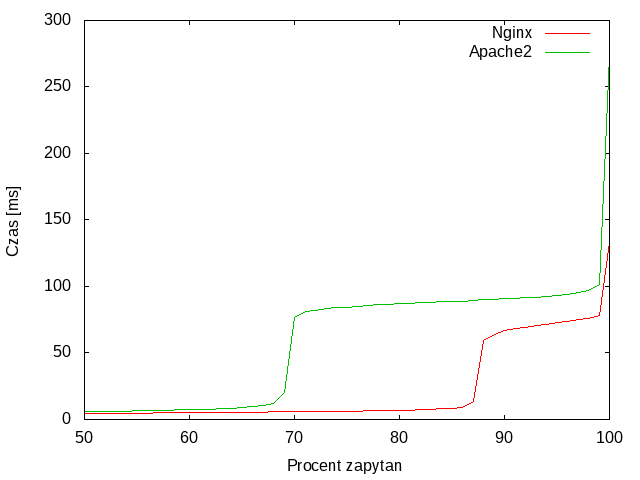
\includegraphics[width=\textwidth]{testy/wybor_index_maly_16.png}
		\caption{16 równoległych zapytań}
	\end{subfigure}
	\begin{subfigure}[h]{0.3\textwidth}
		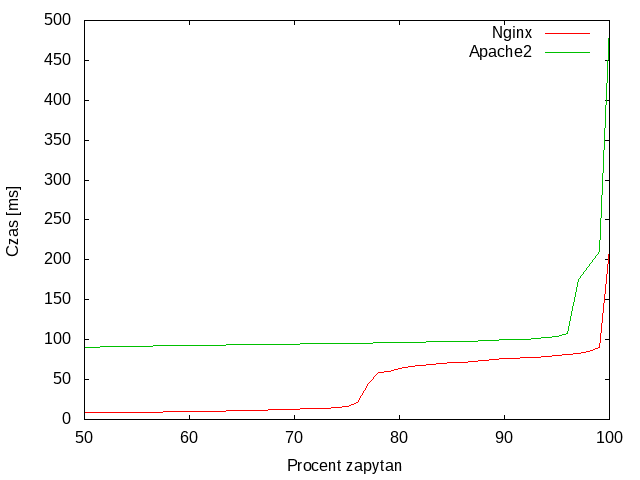
\includegraphics[width=\textwidth]{testy/wybor_index_maly_32.png}
		\caption{32 równoległe zapytania}
	\end{subfigure}

	\begin{subfigure}[h]{0.3\textwidth}
		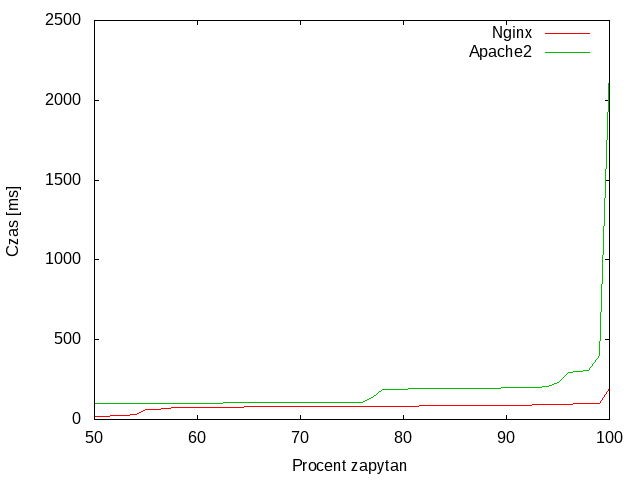
\includegraphics[width=\textwidth]{testy/wybor_index_maly_64.png}
		\caption{64 równoległe zapytania}
	\end{subfigure}
	\begin{subfigure}[h]{0.3\textwidth}
		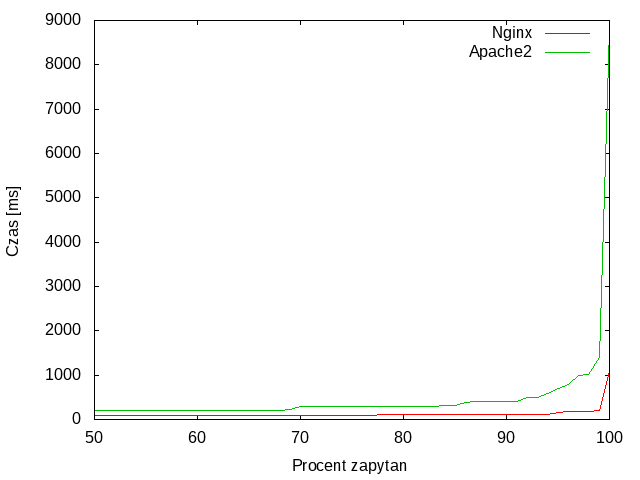
\includegraphics[width=\textwidth]{testy/wybor_index_maly_128.png}
		\caption{128 równoległe zapytania}
	\end{subfigure}
	\begin{subfigure}[h]{0.3\textwidth}
		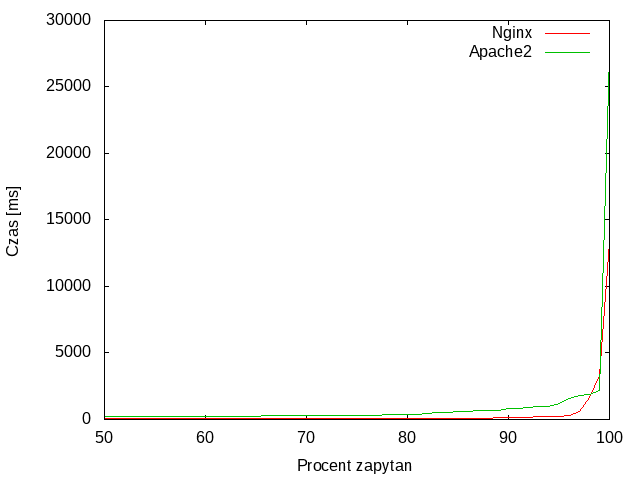
\includegraphics[width=\textwidth]{testy/wybor_index_maly_256.png}
		\caption{256 równoległych zapytań}
	\end{subfigure}
	\caption{Zapytania o mały plik statyczny}\label{fig:wyb_index_maly}
\end{figure}
\begin{figure}
	\centering
	\begin{subfigure}[h]{0.3\textwidth}
		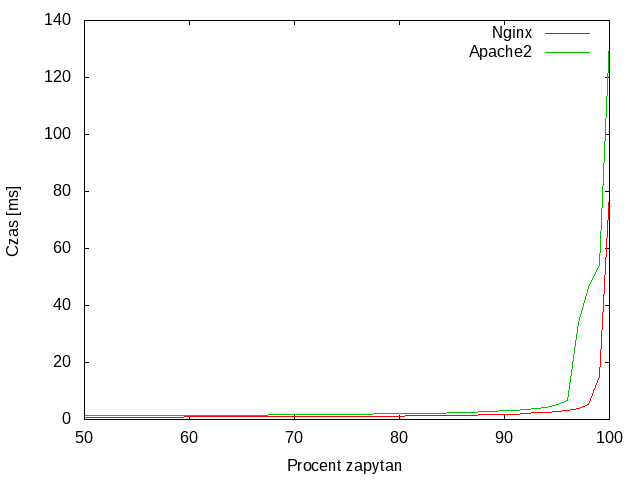
\includegraphics[width=\textwidth]{testy/wybor_index_duzy_1.png}
		\caption{1 równoległe zapytanie}
	\end{subfigure}
	\begin{subfigure}[h]{0.3\textwidth}
		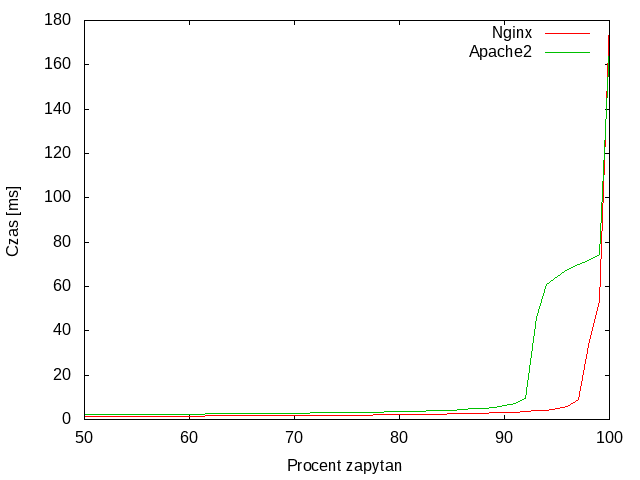
\includegraphics[width=\textwidth]{testy/wybor_index_duzy_2.png}
		\caption{2 równoległe zapytania}
	\end{subfigure}
	\begin{subfigure}[h]{0.3\textwidth}
		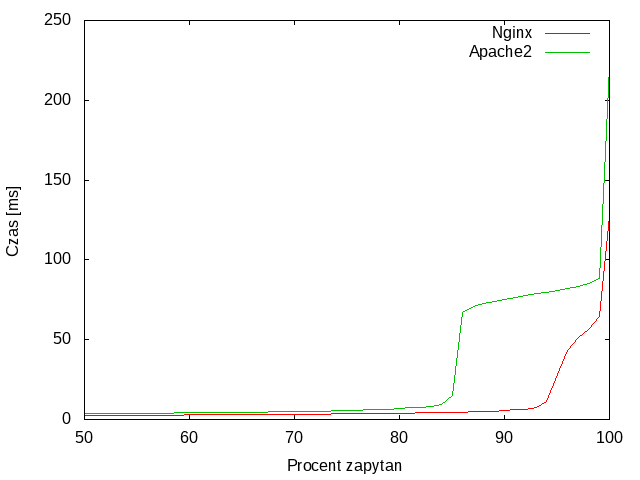
\includegraphics[width=\textwidth]{testy/wybor_index_duzy_4.png}
		\caption{4 równoległe zapytania}
	\end{subfigure}

	\begin{subfigure}[h]{0.3\textwidth}
		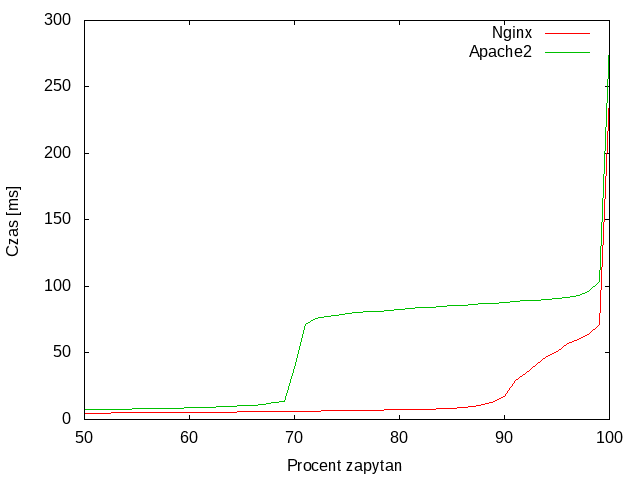
\includegraphics[width=\textwidth]{testy/wybor_index_duzy_8.png}
		\caption{8 równoległych zapytań}
	\end{subfigure}
	\begin{subfigure}[h]{0.3\textwidth}
		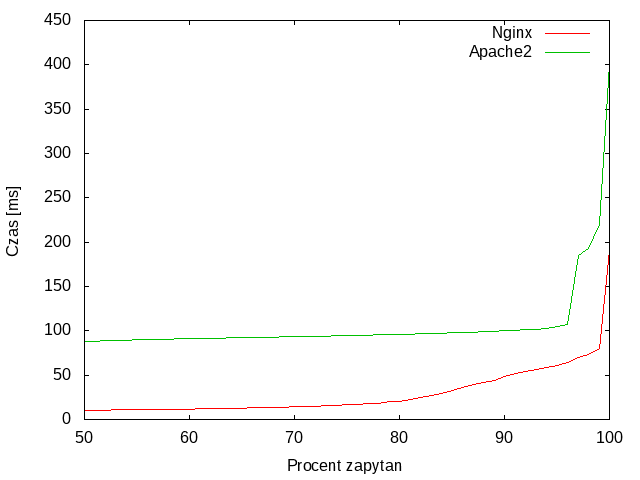
\includegraphics[width=\textwidth]{testy/wybor_index_duzy_16.png}
		\caption{16 równoległych zapytań}
	\end{subfigure}
	\begin{subfigure}[h]{0.3\textwidth}
		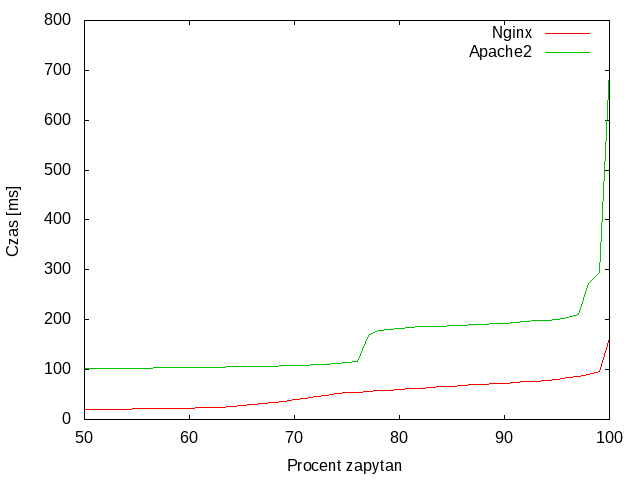
\includegraphics[width=\textwidth]{testy/wybor_index_duzy_32.png}
		\caption{32 równoległe zapytania}
	\end{subfigure}

	\begin{subfigure}[h]{0.3\textwidth}
		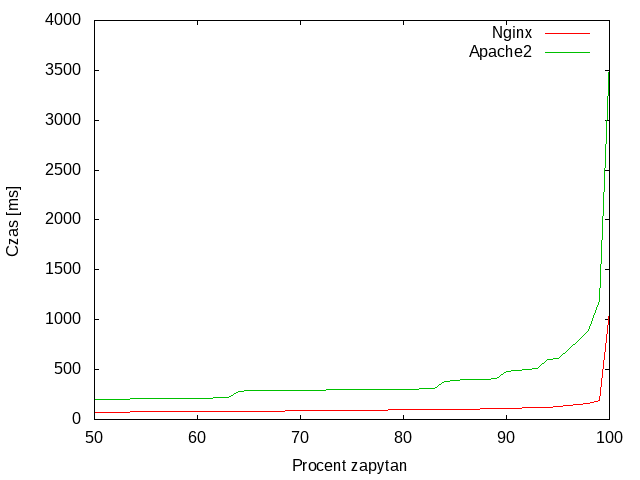
\includegraphics[width=\textwidth]{testy/wybor_index_duzy_64.png}
		\caption{64 równoległe zapytania}
	\end{subfigure}
	\begin{subfigure}[h]{0.3\textwidth}
		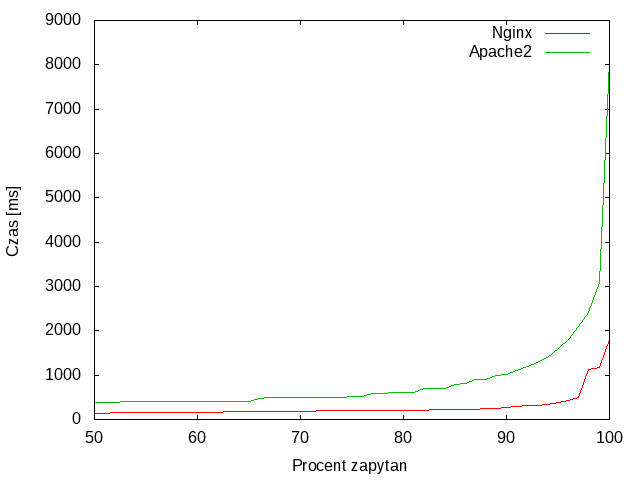
\includegraphics[width=\textwidth]{testy/wybor_index_duzy_128.png}
		\caption{128 równoległe zapytania}
	\end{subfigure}
	\begin{subfigure}[h]{0.3\textwidth}
		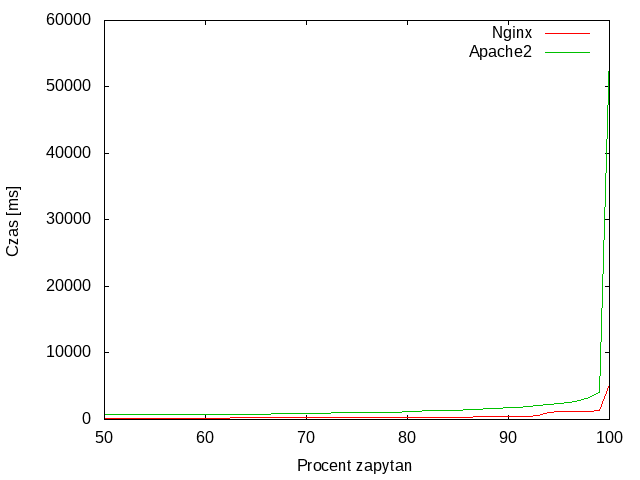
\includegraphics[width=\textwidth]{testy/wybor_index_duzy_256.png}
		\caption{256 równoległych zapytań}
	\end{subfigure}
	\caption{Zapytania o duży plik statyczny}\label{fig:wyb_index_duzy}
\end{figure}
Wykresy na rys.~\ref{fig:wyb_index_maly} przedstawiają czasy obsłużenia zapytań o plik HTML o rozmiarze 10 bajtów, natomiast wykresy na rys.~\ref{fig:wyb_index_duzy} czasy zapytań o plik o rozmiarze 100 kilobajtów.\\
Można zauważyć, że wyniki dla małych plików statycznych są zbliżone zarówno dla Apache jak i Nginx z lekką przewagą dla Nginx.
Największą przewagę Nginx-a widać przy średnim i dużym obciążeniu.
\clearpage
\subsection{Treść dynamiczna}
Testy treści dynamicznej przeprowadzane są przy użyciu konfiguracji Nginx + php-fpm oraz Apache + php-fpm.
Konfiguracja Apache + mod\_php została odrzucona, ponieważ wymaga umieszczenia serwera WWW oraz serwera PHP na jednym serwerze, co uniemożliwia użycie wielu serwerów PHP dla jednego serwera WWW.\\
Do testów zostały wykorzystane dwa bliźniacze skrypty obliczające liczby ciągu Fibonacciego.
Jeden ze skryptów został przedstawiony na listingu~\ref{lst:fib}.
Obliczane są wyrazy: piąty --- dla skryptu wykonującego się szybko, oraz piętnasty --- dla skryptu wykonującego się dłużej.\\
Wykorzystany został model obliczanie wartości rekurencyjny, ponieważ w przeciwieństwie do iteracyjnego wymaga większej mocy obliczeniowej.
Jest to pożądane aby czas obsługi zapytania obejmował czas wykonywania skryptu, a nie jedynie obsługi sesji HTTP oraz transferu danych (zostało to przetestowane przy wykorzystaniu \textit{szybkiego skryptu}).
\lstinputlisting[caption=fib.php,label=lst:fib,language=php]{lst/fib.php}
\begin{figure}
	\centering
	\begin{subfigure}[h]{0.3\textwidth}
		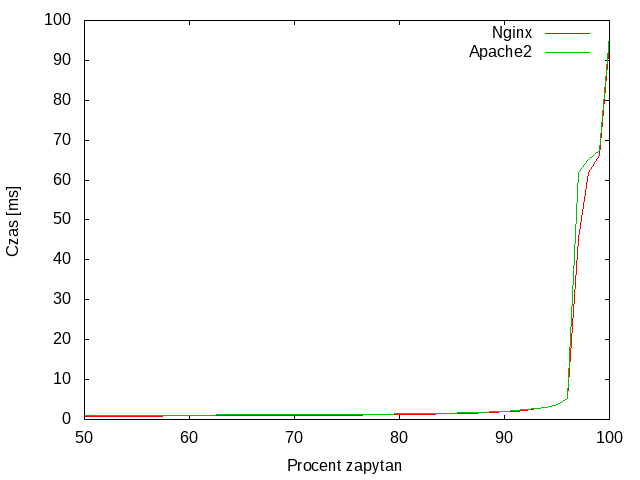
\includegraphics[width=\textwidth]{testy/wybor_fib_5_1.png}
		\caption{1 równoległe zapytanie}
	\end{subfigure}
	\begin{subfigure}[h]{0.3\textwidth}
		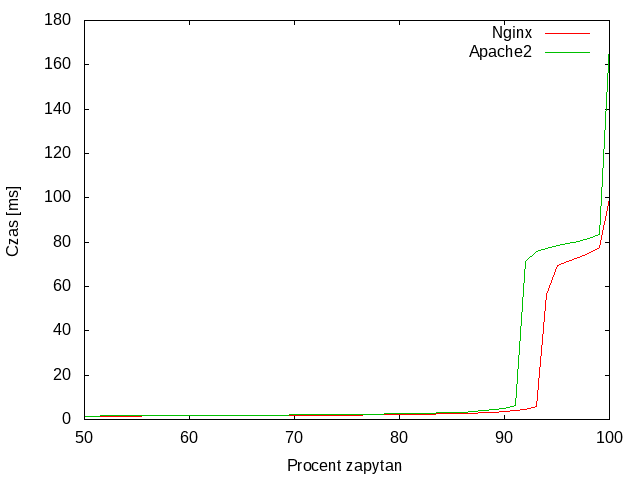
\includegraphics[width=\textwidth]{testy/wybor_fib_5_2.png}
		\caption{2 równoległe zapytania}
	\end{subfigure}
	\begin{subfigure}[h]{0.3\textwidth}
		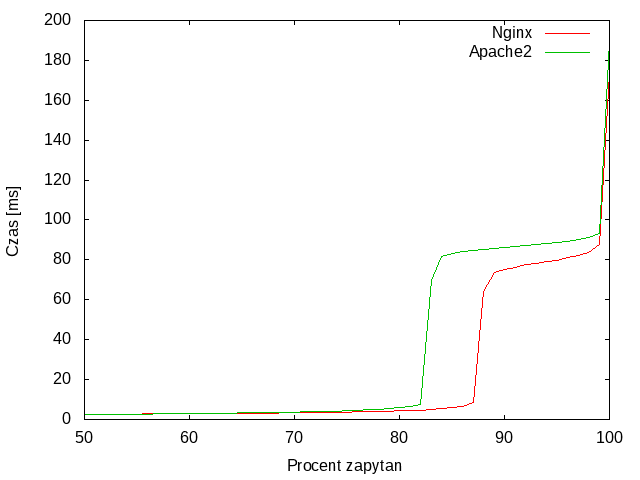
\includegraphics[width=\textwidth]{testy/wybor_fib_5_4.png}
		\caption{4 równoległe zapytania}
	\end{subfigure}

	\begin{subfigure}[h]{0.3\textwidth}
		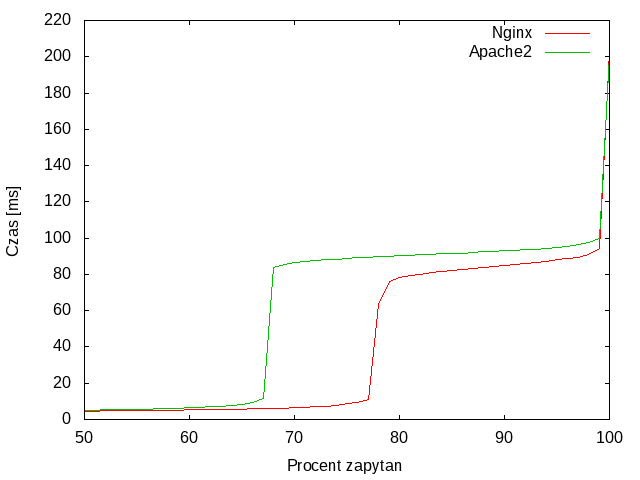
\includegraphics[width=\textwidth]{testy/wybor_fib_5_8.png}
		\caption{8 równoległych zapytań}
	\end{subfigure}
	\begin{subfigure}[h]{0.3\textwidth}
		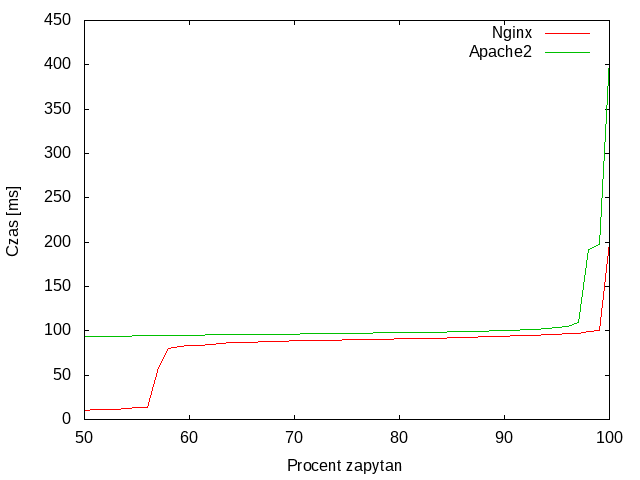
\includegraphics[width=\textwidth]{testy/wybor_fib_5_16.png}
		\caption{16 równoległych zapytań}
	\end{subfigure}
	\begin{subfigure}[h]{0.3\textwidth}
		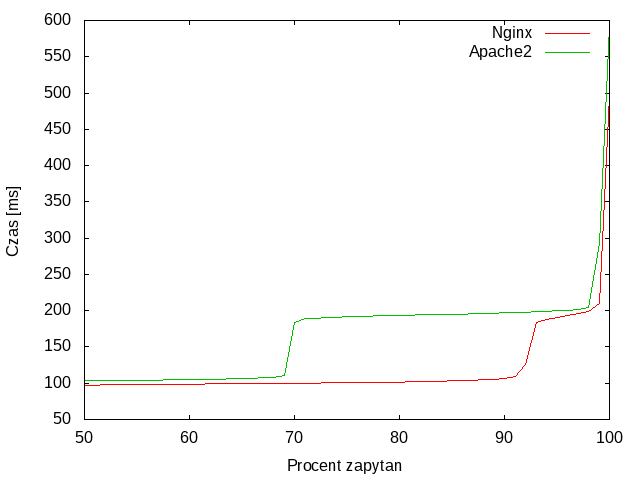
\includegraphics[width=\textwidth]{testy/wybor_fib_5_32.png}
		\caption{32 równoległe zapytania}
	\end{subfigure}

	\begin{subfigure}[h]{0.3\textwidth}
		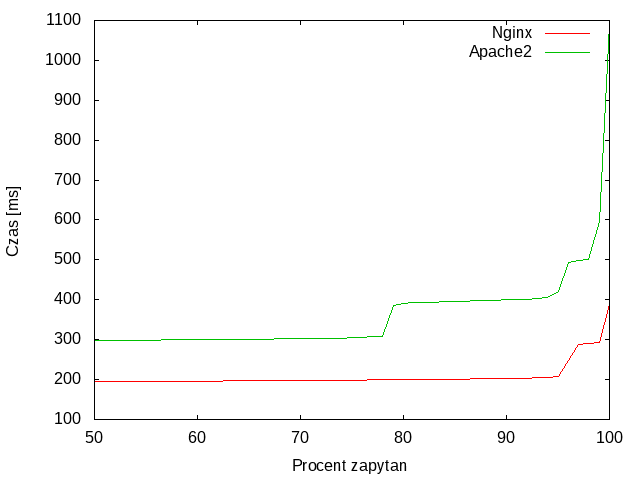
\includegraphics[width=\textwidth]{testy/wybor_fib_5_64.png}
		\caption{64 równoległe zapytania}
	\end{subfigure}
	\begin{subfigure}[h]{0.3\textwidth}
		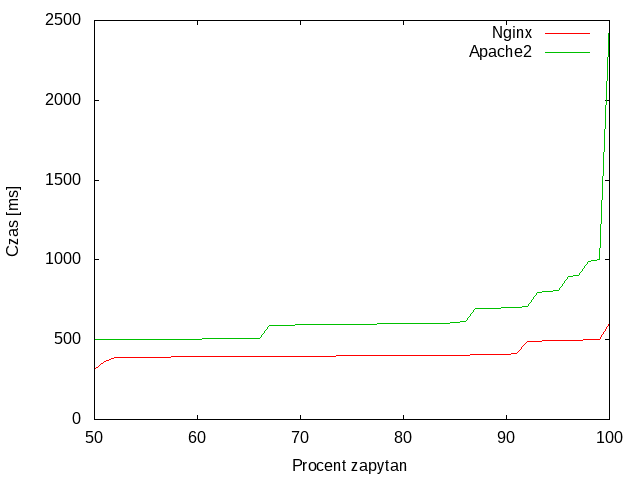
\includegraphics[width=\textwidth]{testy/wybor_fib_5_128.png}
		\caption{128 równoległe zapytania}
	\end{subfigure}
	\begin{subfigure}[h]{0.3\textwidth}
		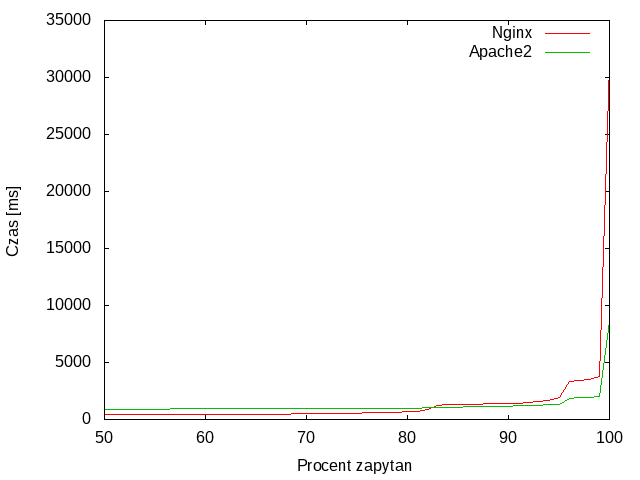
\includegraphics[width=\textwidth]{testy/wybor_fib_5_256.png}
		\caption{256 równoległych zapytań}
	\end{subfigure}
	\caption{Zapytania o szybki skrypt PHP}\label{fig:wyb_fib_5}
\end{figure}
\begin{figure}
	\centering
	\begin{subfigure}[h]{0.3\textwidth}
		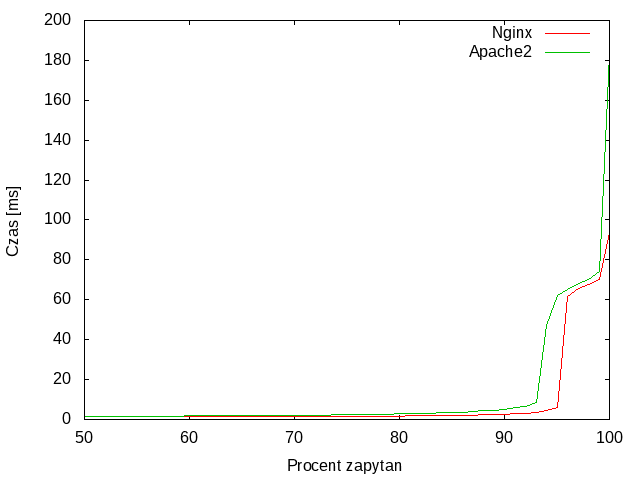
\includegraphics[width=\textwidth]{testy/wybor_fib_15_1.png}
		\caption{1 równoległe zapytanie}
	\end{subfigure}
	\begin{subfigure}[h]{0.3\textwidth}
		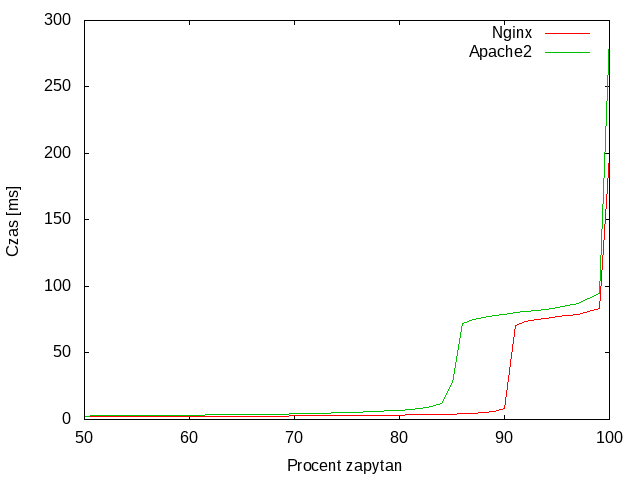
\includegraphics[width=\textwidth]{testy/wybor_fib_15_2.png}
		\caption{2 równoległe zapytania}
	\end{subfigure}
	\begin{subfigure}[h]{0.3\textwidth}
		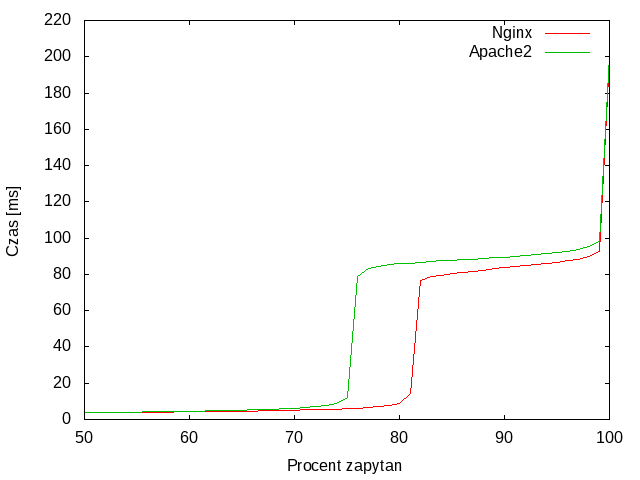
\includegraphics[width=\textwidth]{testy/wybor_fib_15_4.png}
		\caption{4 równoległe zapytania}
	\end{subfigure}

	\begin{subfigure}[h]{0.3\textwidth}
		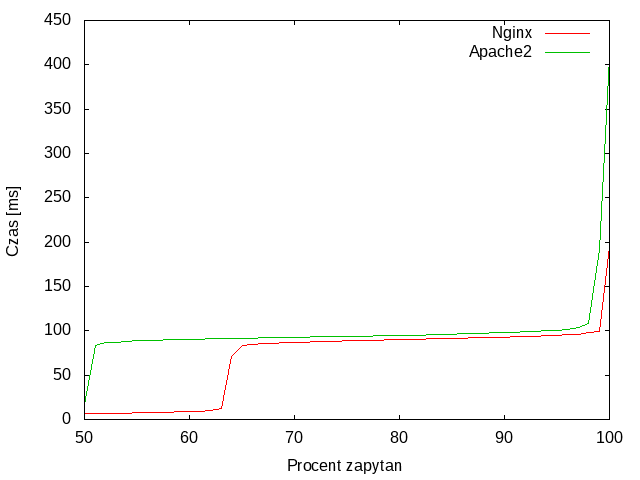
\includegraphics[width=\textwidth]{testy/wybor_fib_15_8.png}
		\caption{8 równoległych zapytań}
	\end{subfigure}
	\begin{subfigure}[h]{0.3\textwidth}
		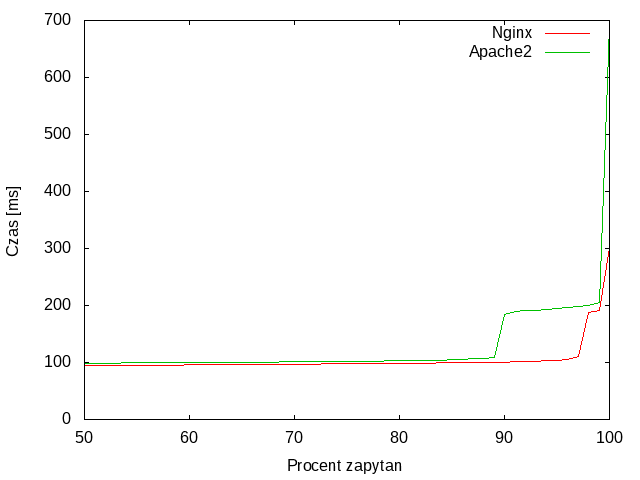
\includegraphics[width=\textwidth]{testy/wybor_fib_15_16.png}
		\caption{16 równoległych zapytań}
	\end{subfigure}
	\begin{subfigure}[h]{0.3\textwidth}
		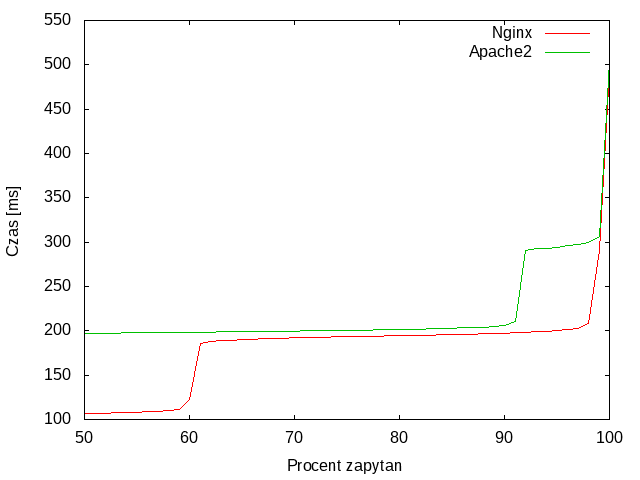
\includegraphics[width=\textwidth]{testy/wybor_fib_15_32.png}
		\caption{32 równoległe zapytania}
	\end{subfigure}

	\begin{subfigure}[h]{0.3\textwidth}
		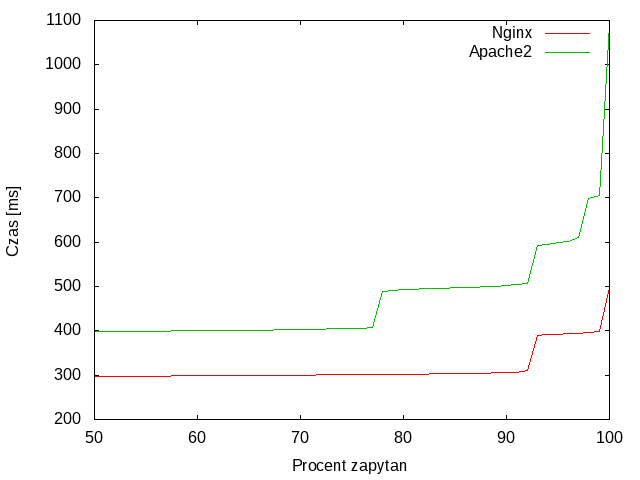
\includegraphics[width=\textwidth]{testy/wybor_fib_15_64.png}
		\caption{64 równoległe zapytania}
	\end{subfigure}
	\begin{subfigure}[h]{0.3\textwidth}
		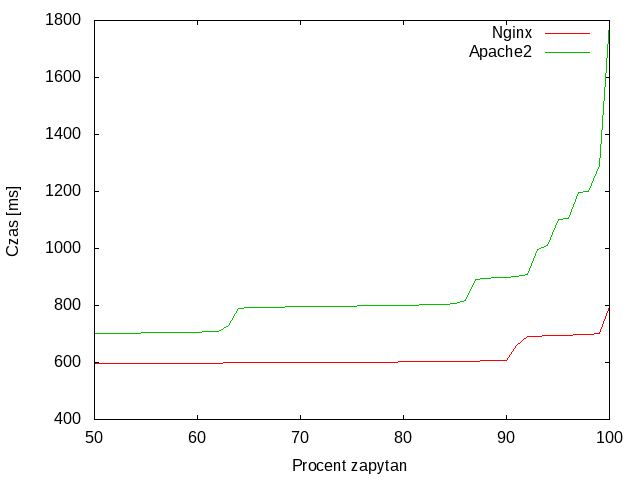
\includegraphics[width=\textwidth]{testy/wybor_fib_15_128.png}
		\caption{128 równoległe zapytania}
	\end{subfigure}
	\begin{subfigure}[h]{0.3\textwidth}
		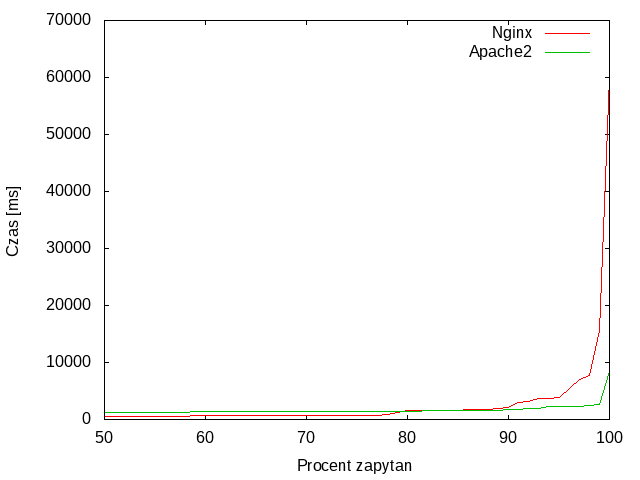
\includegraphics[width=\textwidth]{testy/wybor_fib_15_256.png}
		\caption{256 równoległych zapytań}
	\end{subfigure}
	\caption{Zapytania o wolny skrypt PHP}\label{fig:wyb_fib_15}
\end{figure}
Na wykresach~\ref{fig:wyb_fib_5} oraz~\ref{fig:wyb_fib_15} obrazujących czasy obsługi zapytań do skryptów PHP, można zauważyć że różnice pomiędzy Apache a Nginx są mniejsze niż dla plików statycznych.
Wynika to z faktu, ze obsługą zapytań w obu przypadkach zajmuje się PHP-fpm, natomiast serwer WWW odpowiedzialny jest jedynie za przekazywanie zapytań do \textit{backendu}.
\subsection{Podsumowanie}
Jak wykazały testy, Nginx daje krótsze czasy odpowiedzi we wszystkich testowanych sytuacjach, dlatego został wybrany jako podstawowy serwer wykorzystywany w przedstawionym projekcie.
